\documentclass[12pt,a4paper]{article}
\usepackage[utf8]{inputenc}
\usepackage[T1]{fontenc}
\usepackage[portuguese]{babel}
\usepackage{graphicx}
\usepackage{amsmath}
\usepackage{hyperref}
\usepackage{geometry}
\geometry{a4paper, margin=2.5cm}

\begin{document}

% --- PÁGINA DE ROSTO (Página 1) ---
\begin{titlepage}
    \centering
    \vspace*{1cm}
    
    % Substitui 'logo_iscte.png' pelo nome exato do ficheiro
    
\includegraphics[width=6cm]{logo_iscte.png} 
    
    \vspace{1.5cm}
    {\Large \textbf{Mestrado em Engenharia de Telecomunicações e Informática}}\\[5pt]
    {\large Segurança em Redes e Sistemas de Informação}\par
    
    \vspace{1.5cm}
    {\LARGE \bfseries Deteção de Anomalias e Redução de Falsos Positivos em Ambientes SIEM: Modelação Estatística de Ataques de Força Bruta\par}
    \vspace{1.5cm}
    
    {\Large \textbf{Autores:}}\\[10pt]
    {\large Tomás Cerveira, 122617}\\[5pt]
    {\large Alexandre Duarte, 122657}\\[5pt]
    {\large Lara Machado, 122655}\\[5pt]
    {\large Eduardo Real, 122608}\par
    \vspace{1.5cm}
    
    {\large \textbf{Docentes:}\\ Daniel Pesqueira Morgado e Daniel Maximino Caçador}\par

\vspace{1cm}
    {\normalsize \textbf{Repositório do Projeto (GitHub):}\\ \url{https://github.com/LETI-122617/ISCTE-SIEM-Deteccao-Anomalias}}\par
    
    \vfill
    {\large 30-10-2026\par}
\end{titlepage}

% --- RESUMO E PALAVRAS-CHAVE (Página 2) ---
\newpage
\thispagestyle{plain}
\section*{Resumo}
\addcontentsline{toc}{section}{Resumo}
Os Centros de Operações de Segurança (SOC) enfrentam diariamente o desafio de processar grandes volumes de alertas gerados por sistemas de monitorização, sendo muitos destes alertas considerados falsos positivos que não representam ameaças reais. Este cenário gera "fadiga de alertas" e prejudica a capacidade de resposta a incidentes críticos. O presente trabalho aborda o problema da redução de falsos positivos em ambientes de Security Information and Event Management (SIEM), propondo a substituição de regras analíticas baseadas em limites estáticos por modelos de deteção adaptativos. Através da utilização de formulações estatísticas de média móvel e desvio padrão sobre eventos de autenticação, o estudo conceptualiza a diferenciação entre anomalias genuínas (ataques de força bruta a simular na Parte 2) e o ruído operacional normal da rede. A metodologia assentou numa revisão sistemática da literatura suportada pela plataforma Parsifal. A análise comparativa de 6 estudos de ponta indicou a viabilidade teórica da aplicação de métodos matemáticos (\textit{Z-scores} e limiares adaptativos) na redução estatística de alarmes falsos. Esta abordagem nativa apresenta o potencial de contornar as latências proibitivas e as elevadas taxas de falsos positivos associadas a arquiteturas computacionalmente pesadas, como os \textit{Large Language Models} (LLMs), estabelecendo as bases para a futura validação empírica.

\vspace{1em}
\noindent\textbf{Palavras-chave:} SIEM, Falsos Positivos, Deteção de Anomalias, Força Bruta, SOC, Modelos Estatísticos.

% --- ÍNDICE (Página 3) ---
\newpage
\renewcommand{\contentsname}{Índice}
\tableofcontents

% --- CORPO DO DOCUMENTO (Página 4 em diante) ---
\newpage

\section*{Glossário}
\addcontentsline{toc}{section}{Glossário}
\begin{itemize}
    \item \textbf{CMDB} -- Configuration Management Database
    \item \textbf{EC} -- Exclusion Criteria (Critério de Exclusão)
    \item \textbf{FN} -- \textit{False Negative} (Falso Negativo)
    \item \textbf{FP} -- \textit{False Positive} (Falso Positivo)
    \item \textbf{FPR} -- False Positive Rate
    \item \textbf{IAM} -- Identity and Access Management
    \item \textbf{IC} -- Inclusion Criteria (Critério de Inclusão)
    \item \textbf{IDS} -- Intrusion Detection System
    \item \textbf{KQL} -- Kibana Query Language
    \item \textbf{LLM} -- Large Language Model
    \item \textbf{MAD} -- Median Absolute Deviation (Desvio Absoluto da Mediana)
    \item \textbf{MITRE ATT\&CK} -- Adversarial Tactics, Techniques, and Common Knowledge
    \item \textbf{ML} -- Machine Learning
    \item \textbf{ROC-AUC} -- Receiver Operating Characteristic - Area Under Curve
    \item \textbf{RQ} -- Research Question (Questão de Pesquisa)
    \item \textbf{SIEM} -- Security Information and Event Management
    \item \textbf{SOC} -- Security Operations Center
    \item \textbf{SPL} -- Search Processing Language
    \item \textbf{SSH} -- Secure Shell
    \item \textbf{TCS} -- Threat Confidence Score
    \item \textbf{TN} -- \textit{True Negative} (Negativo Verdadeiro)
    \item \textbf{TP} -- \textit{True Positive} (Positivo Verdadeiro)
\end{itemize}

\newpage

\section{Introdução}
A capacidade de monitorizar redes e sistemas informáticos em tempo real é um pilar fundamental da cibersegurança. No entanto, existe um problema crítico relacionado com a eficácia das ferramentas de monitorização: a geração de um grande volume de alertas que não representam a real situação do ambiente computacional, dificultando a análise feita pelos administradores de sistemas. Estes falsos positivos obrigam as equipas de analistas a desperdiçar recursos na triagem de eventos benignos, atrasando a resposta a verdadeiros incidentes de segurança.

Este projeto visa resolver o problema da ineficiência na deteção de intrusões provocada por regras de alerta estáticas. Como a literatura recente demonstra, a adoção de Inteligência Artificial massiva (como LLMs) para tentar solucionar este problema tem introduzido latências incompatíveis com o processamento em tempo real e agravado as taxas de falsos positivos (FPR) devido ao viés computacional. Para endereçar este desafio de forma otimizada, propõe-se o estudo e fundamentação teórica de um modelo adaptativo num ambiente SIEM, focado na aplicação nativa de funções matemáticas e estatísticas descritivas para estabelecer \textit{baselines} de comportamento normal na rede. Ao conceptualizar o cálculo de desvios padrão dinâmicos e \textit{Z-scores}, procura-se avaliar em que medida o sistema pode filtrar o ruído benigno e identificar ataques de força bruta com um custo computacional residual.

O documento encontra-se estruturado da seguinte forma: a Secção 2 apresenta a fundamentação teórica, detalhando a arquitetura SIEM e o impacto da fadiga de alertas num SOC; a Secção 3 detalha a revisão sistemática da literatura e o estado da arte das abordagens de mitigação de ruído; por fim, a Secção 4 expõe as conclusões teóricas alcançadas e os trabalhos futuros delineados para o desenvolvimento prático deste projeto.

\newpage

\section{Fundamentação Teórica}
\subsection{Security Operations Centers e a Plataforma SIEM}
Os \textit{Security Operations Centers} (SOCs) desempenham um papel crítico na cibersegurança das organizações, garantindo a monitorização contínua, deteção e resposta a incidentes. O núcleo tecnológico destas operações assenta em plataformas \textit{Security Information and Event Management} (SIEM), que agregam volumes massivos de dados provenientes de sistemas de deteção e prevenção de intrusões (IDS/IPS) \cite{roy2026}. 

Contudo, o crescimento exponencial do volume de dados gerados tem provocado um fenómeno severo de fadiga de alertas (\textit{alert fatigue}) entre as equipas de analistas. Este problema é impulsionado, na sua grande maioria, por elevadas taxas de falsos positivos resultantes de regras de deteção estáticas que carecem de contexto organizacional. A literatura demonstra a escala operacional deste desafio: os analistas operam sob intensa pressão temporal, conseguindo rever apenas uma fração dos alertas \cite{rieger2026, roy2026}. O impacto é massivo, uma vez que as operações de SOC recebem frequentemente mais de 10.000 eventos diários, estimando-se que cerca de 90\% destes registos representem falsos positivos \cite{yauri2026}. A ausência de adaptação dinâmica aos padrões de atividade normal da rede torna a monitorização ineficiente, resultando em respostas atrasadas, incidentes ignorados e exaustão psicológica das equipas de segurança \cite{rieger2026}.

\subsection{Modelação Matemática da Deteção}
Para colmatar as falhas das abordagens baseadas em limites estáticos e evitar a sobrecarga de arquiteturas \textit{black-box} de inteligência artificial, a nossa proposta teórica assenta na identificação de anomalias através da estatística descritiva aplicada nativamente aos \textit{logs} do SIEM. Esta lógica assemelha-se à modelação de desvios padronizados (\textit{Z-scores}) demonstrada por Mohanapriya et al. (2026), mas calculada em tempo real sobre séries temporais de eventos.

O volume de eventos de autenticação falhados num instante $t$, denotado por $X_t$, é avaliado em relação ao histórico de tráfego. A média móvel ($\mu$) e o desvio padrão ($\sigma$) para uma janela de tempo com $N$ observações anteriores (excluindo propositadamente o instante atual $X_t$ no somatório de $i=1$ a $N$, para que o pico anómalo não mascare a própria \textit{baseline}) são calculados através das seguintes formulações matemáticas:
\begin{equation}
    \mu = \frac{1}{N} \sum_{i=1}^{N} X_{t-i}
\end{equation}

\begin{equation}
    \sigma = \sqrt{\frac{1}{N} \sum_{i=1}^{N} (X_{t-i} - \mu)^2}
\end{equation}

Com base nestas métricas, o desvio normalizado (\textit{Z-score}) do tráfego atual é calculado para quantificar a distância do evento face ao comportamento esperado. Para evitar indeterminações matemáticas em janelas de tempo com tráfego perfeitamente constante (onde $\sigma = 0$), introduz-se uma constante residual $\epsilon$ (e.g., $\epsilon = 1$, garantindo um limite mínimo de variação natural aceitável):
\begin{equation}
    Z_t = \frac{X_t - \mu}{\sigma + \epsilon}
\end{equation}

Um alerta é acionado, indicando um potencial ataque de força bruta, se o desvio atual ultrapassar uma constante de limiar $k$ (onde $Z_t > k$). Matematicamente, resolvendo a inequação para o volume de eventos no SIEM, obtemos o critério direto de deteção da nossa arquitetura:
\begin{equation}
    X_t > \mu + k\sigma
\end{equation}

A constante $k$ atua como o calibrador de sensibilidade do SOC, sendo tipicamente definida com o valor 3, baseando-se na regra empírica da estatística para abranger 99,7\% do tráfego legítimo esperado. Refira-se que esta formulação assume uma distribuição aproximadamente normal das contagens de eventos, premissa que será validada com dados reais na Parte 2 do projeto. 

Reconhece-se ainda a limitação inerente da contaminação da \textit{baseline}: um ataque lento e prolongado (\textit{low and slow}) pode inflacionar gradualmente os valores de $\mu$ e $\sigma$, mascarando a anomalia. Em trabalhos futuros, esta lacuna poderá ser mitigada pela exclusão de pontos já sinalizados da janela temporal ou pelo uso do Desvio Absoluto da Mediana (MAD). Do ponto de vista operacional, o cálculo contínuo destas métricas pode ser implementado de forma nativa através de linguagens de pesquisa do SIEM, como o \textit{Search Processing Language} (SPL) no Splunk (recorrendo ao comando \texttt{streamstats}) ou o \textit{Kibana Query Language} (KQL) na \textit{Elastic Stack}, dispensando \textit{hardware} dedicado.

\begin{figure}[h]
    \centering
    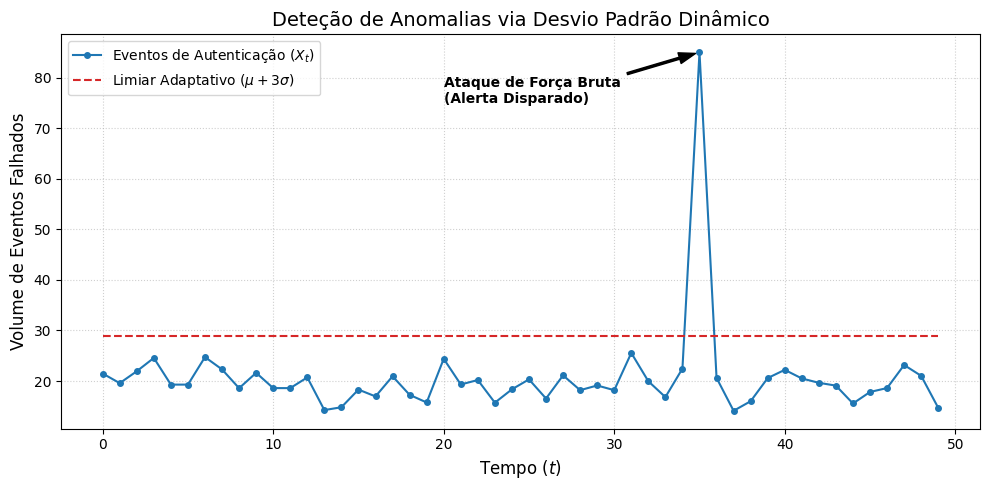
\includegraphics[width=0.85\textwidth]{grafico_limiar.png}
    \caption{Representação conceptual do limiar adaptativo ($\mu + k\sigma$) a isolar um pico anómalo de eventos de autenticação num SOC.}
    \label{fig:grafico_limiar}
\end{figure}

\subsection{Métricas de Avaliação de Desempenho}
Para validar a eficácia do modelo estatístico proposto e permitir uma comparação justa com as abordagens de \textit{Machine Learning} identificadas no estado da arte, o desempenho da deteção deve ser medido recorrendo à matriz de confusão. A avaliação da eficácia na redução de falsos positivos num SOC baseia-se nas seguintes métricas matemáticas:

\textbf{Precisão (\textit{Precision}):} Avalia a proporção de alertas classificados como anómalos que correspondem a verdadeiros ataques, mitigando o ruído operacional:
\begin{equation}
    Precision = \frac{TP}{TP + FP}
\end{equation}

\textbf{Sensibilidade (\textit{Recall}):} Mede a capacidade do modelo em detetar a totalidade das ameaças reais, garantindo que incidentes críticos não são ignorados:
\begin{equation}
    Recall = \frac{TP}{TP + FN}
\end{equation}

\textbf{Especificidade (\textit{Specificity}):} Quantifica a capacidade do sistema em classificar corretamente o tráfego benigno, essencial para não gerar falsos alarmes:
\begin{equation}
    Specificity = \frac{TN}{TN + FP}
\end{equation}

\textbf{\textit{F-Score}:} Representa a média harmónica entre a Precisão e a Sensibilidade. Num ambiente SIEM, caracterizado por um forte desbalanceamento de classes (onde o volume de eventos benignos é ordens de grandeza superior ao de ataques), esta métrica é um dos indicadores mais robustos para avaliar o modelo:
\begin{equation}
    F\text{-}Score = 2 \times \frac{Precision \times Recall}{Precision + Recall}
\end{equation}

\section{Estado da Arte e Revisão Sistemática}
Para compreender as abordagens atuais à redução de alertas, foi elaborado um protocolo de revisão sistemática de literatura, definindo o problema, questões de pesquisa principais e estatísticas. A pesquisa foi conduzida em bases de dados bibliográficas, tendo os estudos sido selecionados através de rigorosos critérios de inclusão e exclusão filtrados pelo título e \textit{abstract}.

\begin{figure}[h]
    \centering
    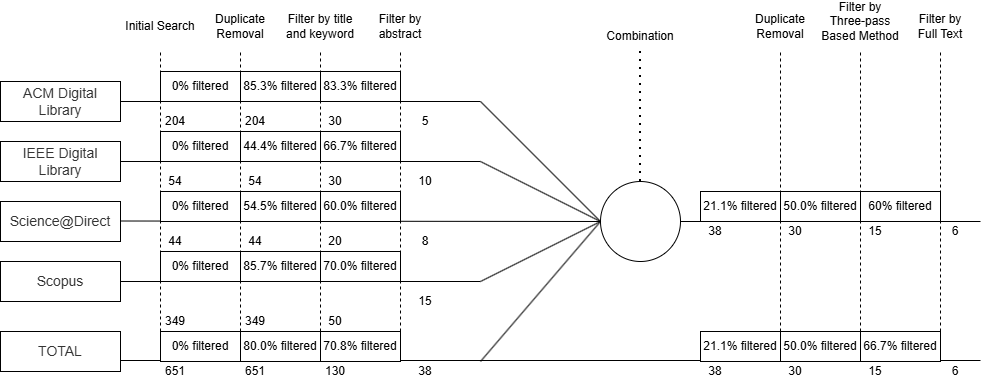
\includegraphics[width=\textwidth]{diagrama_pesquisa.png}
    \caption{Fluxo do processo de seleção de estudos da revisão sistemática da literatura.}
    \label{fig:fluxo_revisao}
\end{figure}

Para garantir o rigor metodológico, a revisão seguiu diretrizes estruturadas na plataforma Parsifal. A investigação foi norteada por duas Questões de Pesquisa (RQ) fundamentais: \textbf{RQ1:} Quais as limitações operacionais das soluções baseadas em IA (ML e LLMs) num SOC? \textbf{RQ2:} Como podem os modelos estatísticos adaptativos otimizar a redução de falsos positivos? 

A extração de dados incidiu sobre publicações da última década (2016-2026), utilizando a \textit{string} de busca: \texttt{("SIEM" OR "SOC") AND ("false positive*" OR "alert fatigue") AND ("anomaly detection" OR "statistical modeling")}. Aplicou-se um Critério de Inclusão (\textbf{IC1}): estudos com foco explícito em ambientes SIEM, redução de fadiga de alertas ou modelação de anomalias em tráfego de rede. 

O processo de triagem (Figura \ref{fig:fluxo_revisao}) iniciou-se com 651 artigos recolhidos de bases de dados científicas (ACM, IEEE, ScienceDirect e Scopus). Numa primeira fase local de remoção de duplicados, não se registaram exclusões, transitando os 651 artigos para a filtragem por título e palavras-chave, que reduziu a amostra substancialmente para 130 documentos. A subsequente filtragem por \textit{abstract} isolou 38 artigos. Após a combinação dos resultados das quatro bases, realizou-se uma segunda remoção de duplicados globais (restando 30 artigos), seguida de uma triagem pelo método de três passagens (\textit{Three-pass Based Method}), que reduziu o conjunto para 15 trabalhos. Por fim, na fase de leitura integral (\textit{Full Text}), aplicaram-se dois Critérios de Exclusão (EC) principais: \textbf{EC1} rejeitou trabalhos fora do âmbito de TI tradicional (e.g., redes de água ou IoT industrial); \textbf{EC2} excluiu publicações puramente teóricas ou focadas em partilha federada sem métricas de mitigação de ruído. Este processo iterativo e rigoroso culminou na seleção final de 6 estudos para análise aprofundada.

\subsection{Abordagens Atuais na Redução de Falsos Positivos}
Para mitigar a fadiga de alertas, a comunidade académica tem explorado soluções avançadas que visam injetar contexto e dinamicidade na classificação de eventos. Trabalhos de referência exploram a aplicação de algoritmos de aprendizado de máquina supervisionado aliados ao enriquecimento de atributos organizacionais. Moraes et al. (2017) propuseram uma arquitetura de duas fases aplicada aos \textit{logs} de um IDS Snort: primeiramente, os alertas informativos de baixa prioridade (prioridade 3) são filtrados de forma estática, o que num estudo de caso real reduziu o volume bruto de mais de 2,2 milhões de alertas mensais para cerca de 26 mil \cite{moraes2017}. Numa segunda fase, os alertas críticos sobreviventes são enriquecidos com dados externos (como geolocalização via \textit{GeoIP}) e topologia da rede (papel e função do \textit{host}) \cite{moraes2017}. Ao submeter estes dados a classificadores, o estudo demonstrou que o algoritmo \textit{Random Forest} supera o \textit{k-Nearest Neighbors} (kNN) na robustez perante o desbalanceamento de classes, alcançando taxas de precisão, sensibilidade e especificidade sistematicamente entre os 95,08\% e os 100\% na identificação final de falsos positivos \cite{moraes2017}. 

Expandindo a aplicação empírica de Inteligência Artificial, Yauri et al. (2026) avaliaram o desempenho de modelos de \textit{Machine Learning} (ML) processando 98.321 registos reais extraídos de uma firewall Palo Alto num ambiente SIEM \cite{yauri2026}. O estudo aplicou técnicas rigorosas de pré-processamento, recorrendo ao agrupamento não supervisionado (\textit{K-Means}) para validação de especialistas, além da transformação de variáveis categóricas utilizando \textit{Weight of Evidence} (WoE) e \textit{Information Value} (IV) \cite{yauri2026}. Após a avaliação e afinação de hiperparâmetros em dez classificadores distintos, o modelo \textit{Gradient Boosting} destacou-se com uma área sob a curva (ROC-AUC) de 0.9964 e um \textit{F1-score} de 97.32\% \cite{yauri2026}. A eficácia da otimização refletiu-se de forma substancial na matriz de confusão: num universo de teste superior a 18.600 eventos, o modelo registou apenas 120 falsos positivos e 259 falsos negativos, validando a capacidade destes algoritmos em filtrar ruído sem comprometer a identificação atempada de incidentes críticos \cite{yauri2026}.

Aprofundando a eficácia das abordagens construídas nativamente em plataformas SIEM, Bhardwaj (2026) propôs uma metodologia de \textit{threat hunting} focada na correlação comportamental para detetar vetores de acesso inicial (como documentos maliciosos e execução de \textit{LOLBins}) operando num ambiente \textit{Elasticsearch} \cite{bhardwaj2026}. O autor desenvolveu um modelo de Pontuação de Confiança de Ameaça (\textit{Threat Confidence Score} - TCS) baseado em pesquisas multicondicionais de linhagem de processos (relação pai-filho e argumentos de linha de comando) \cite{bhardwaj2026}. Num teste empírico que recorreu a telemetria real de produção, o sistema ingeriu exatamente 12.079.598 eventos de \textit{log} \cite{bhardwaj2026}. A aplicação desta lógica de triagem comportamental conseguiu reduzir este volume massivo para apenas 54 potenciais alertas \cite{bhardwaj2026}. Após validação, o modelo confirmou 3 verdadeiros positivos e suprimiu o ruído para apenas 2 falsos positivos, alcançando uma taxa de sensibilidade (\textit{recall}) perfeita de 1.0 e um \textit{F1-score} equilibrado de 75\% \cite{bhardwaj2026}. Embora estes resultados atestem uma elevada fiabilidade na filtragem de ruído sem dependência de algoritmos externos pesados, a limitação operacional desta solução reside na necessidade de desenhar, afinar e manter arquiteturas complexas de regras encadeadas e limiares de risco definidos manualmente por especialistas com base na \textit{framework} MITRE ATT\&CK \cite{bhardwaj2026}.

Em contraponto ao sucesso da modelação comportamental, a aplicação recente de \textit{Large Language Models} (LLMs) na triagem de alertas SIEM tem revelado severas limitações operacionais \cite{rieger2026}. Num estudo comparativo exaustivo, Rieger et al. (2026) avaliaram modelos de ponta (como as famílias GPT-4, DeepSeek e Olmo 3) contra classificadores estatísticos e baseline tradicionais \cite{rieger2026}. Os resultados demonstraram que, embora os LLMs atinjam taxas de sensibilidade elevadas, geram uma quantidade insustentável de ruído e sofrem de sobreclassificação constante \cite{rieger2026}. O modelo \textit{Olmo 3}, por exemplo, registou uma taxa de falsos positivos (FPR) de 90.54\%, enquanto o \textit{GPT-4o-mini} atingiu 72.97\% de FPR, agravando severamente a fadiga de alertas que se propunham resolver \cite{rieger2026}. Além da imprecisão analítica, a latência computacional mostrou-se proibitiva para ambientes reais, com modelos a demorarem até 85.8 segundos (\textit{DeepSeek-Reasoner}) para processar um único alerta \cite{rieger2026}.

Corroborando esta ineficiência e a complexidade operacional dos modelos generativos, Roy e Balde (2026) avaliaram o uso do modelo massivo \textit{Meta LLaMA 3.3-70B} na classificação de alertas de nível 1 num ambiente SIEM Wazuh \cite{roy2026}. A investigação demonstrou que, na ausência de contexto organizacional detalhado, o LLM assume um "viés de cautela" (gerando falsos positivos) e sofre de variabilidade nas suas decisões, alcançando uma precisão de apenas 80\% \cite{roy2026}. Embora os autores provem que a injeção contínua de ficheiros JSON com contexto estruturado consegue mitigar os falsos positivos, esta abordagem exige a integração e manutenção de bases de dados contextuais dinâmicas (como sistemas CMDB e IAM) acopladas a um modelo de 70 mil milhões de parâmetros \cite{roy2026}. 

Em paralelo às abordagens generativas, arquiteturas híbridas como a plataforma GarudanEye, proposta por Mohanapriya et al. (2026), evidenciam o potencial de combinar múltiplos métodos de deteção com modelos matemáticos de desvio \cite{mohanapriya2026}. Processando 2,83 milhões de registos de tráfego de rede, o sistema integra classificação de \textit{Random Forest} com o cálculo de desvios padronizados (\textit{Z-scores}) para estabelecer perfis de anomalias com base na média e no desvio padrão das características da rede \cite{mohanapriya2026}. Esta abordagem híbrida resultou num FPR excecionalmente baixo de 0.0022 e numa precisão global de 96.91\% \cite{mohanapriya2026}, indicando que a identificação de anomalias com base em métodos estatísticos de desvio consegue diferenciar eficazmente o tráfego benigno das instâncias de ataque, mitigando o ruído de alertas com alta eficiência computacional \cite{mohanapriya2026}.

Em suma, a literatura mais recente demonstra que a Inteligência Artificial pesada, embora promissora em testes isolados, introduz dependências arquitetónicas, propensão para falsos positivos e custos computacionais que contrariam a necessidade de agilidade e automação de um SOC. É exatamente para colmatar esta lacuna técnica e estrutural que o presente projeto se insere: em vez de recorrer a modelos \textit{black-box} morosos ou regras encadeadas manuais, propomos o uso nativo do \textbf{Desvio Padrão Dinâmico} e \textbf{Médias Móveis} diretamente no motor de correlação do SIEM. Esta abordagem procura isolar anomalias com um \textit{overhead} esperado reduzido, pretendendo minimizar falsos positivos em tempo real sem \textit{hardware} dispendioso ou treino complexo.

\subsection{Síntese Comparativa}
É crucial salientar que os resultados numéricos reportados na literatura não são diretamente comparáveis de forma absoluta, dado que os estudos utilizam \textit{datasets} (e.g., CICIDS2017 vs. telemetria real fechada), escalas operacionais e métricas primárias de avaliação distintas. Servem, ainda assim, como indicadores do comportamento das arquiteturas. A Tabela \ref{tab:comparativo} resume as metodologias analisadas e evidencia o posicionamento da nossa formulação estatística face às limitações identificadas.

\begin{table}[h]
    \centering
    \caption{Comparativo das Abordagens na Literatura para Redução de Falsos Positivos em SIEM}
    \vspace{0.3cm}
    \resizebox{\textwidth}{!}{%
    \begin{tabular}{|l|l|l|l|l|l|}
    \hline
    \textbf{Estudo} & \textbf{Metodologia / Tecnologia} & \textbf{Dataset / Escala} & \textbf{Métrica Principal} & \textbf{Vantagem Evidenciada} & \textbf{Limitação Operacional (SOC)} \\ \hline
    Moraes et al. (2017) \cite{moraes2017} & Machine Learning (kNN e RF) & Logs Snort (2M alertas) & Precisão $\approx$ 100\% & Excelente classificação estática & Exige extração de dados e treino externo \\ \hline
    Yauri et al. (2026) \cite{yauri2026} & Gradient Boosting & Logs Palo Alto (98K ev.) & ROC-AUC: 0.996 & Alta separação comportamental & Otimização complexa de hiperparâmetros \\ \hline
    Bhardwaj (2026) \cite{bhardwaj2026} & Correlação Comportamental & Telemetria Real (12M logs) & F1-Score: 75\% & Filtra eventos fidedignos de ruído & Requer regras encadeadas complexas \\ \hline
    Rieger et al. (2026) \cite{rieger2026} & LLMs vs. ML (Linear SVM) & Dataset simulado (178 alertas) & FPR: 90.5\% (LLMs) & ML leve supera LLMs na triagem & LLMs geram latência alta (85s) e ruído \\ \hline
    Roy \& Balde (2026) \cite{roy2026} & LLMs (Meta LLaMA 3.3-70B) & Cyber-Range (55 alertas) & Accuracy: 100\% & Injeção direta de contexto & Exige manutenção contínua de bases \\ \hline
    Mohanapriya et al. (2026) \cite{mohanapriya2026} & Híbrida (RF + Z-scores) & CICIDS2017 (2.8M logs) & FPR: 0.0022 & FPR excecionalmente baixo & Requer conjugação de múltiplos motores \\ \hline
    \textbf{Nossa Proposta} & \textbf{Estatística Nativa (Desvio Padrão)} & \textbf{A simular (Parte 2)} & \textbf{A calcular (Parte 2)} & \textbf{Vantagem Esperada:} Baixa latência & \textbf{Âmbito restrito a força bruta} \\ \hline
    \end{tabular}%
    }
    \label{tab:comparativo}
\end{table}

\section{Conclusões e Trabalhos Futuros}
O presente trabalho evidencia, através da revisão sistemática da literatura, que a dependência de assinaturas estáticas na deteção de intrusões contribui severamente para a fadiga de alertas num SOC. O estado da arte indica que, embora abordagens baseadas em inteligência artificial (LLMs e ML complexo) consigam atenuar a taxa de falsos positivos (FPR), estas acarretam complexidade computacional, latências elevadas e necessitam de manutenção manual exaustiva de bases de contexto organizacional. Conclui-se concetualmente que a aplicação nativa de modelos estatísticos dinâmicos diretamente na plataforma SIEM apresenta o potencial de autoajustar limiares, visando suprimir ruído sem introduzir um \textit{overhead} insustentável nas operações.

\textbf{Trabalhos Futuros:}
No âmbito da continuidade deste projeto (Parte 2), a arquitetura teórica proposta será alvo de validação empírica. Os trabalhos futuros focar-se-ão em três eixos centrais:
\begin{enumerate}
    \item \textbf{Implementação Prática:} Materialização do modelo matemático através de \textit{queries} nativas em plataformas reais (e.g., Splunk via SPL ou Elastic Stack via KQL).
    \item \textbf{Simulação e Calibração:} Geração de tráfego benigno mesclado com simulações de ataques de força bruta, procedendo à calibração empírica da janela temporal ($N$) e da constante de sensibilidade ($k$). Adicionalmente, será abordada a mitigação da sazonalidade natural do tráfego (padrões diurnos/noturnos).
    \item \textbf{Avaliação de Desempenho:} Extração das métricas (Precisão, Sensibilidade, Especificidade e \textit{F-Score}) e comparação direta com um cenário de limiares estáticos, \textbf{avaliando} a redução quantitativa da taxa de falsos positivos (FPR).
\end{enumerate}

\newpage
\renewcommand\refname{Referências}
\begin{thebibliography}{9}
\addcontentsline{toc}{section}{Referências}

\bibitem{bhardwaj2026}
Bhardwaj, A. (2026).
\textit{Security framework for threat hunting advanced adversaries for initial level access}. \textit{Computer Networks}, 288, 112630. \url{https://doi.org/10.1016/j.comnet.2026.112630}

\bibitem{mohanapriya2026}
Mohanapriya, D., Dharsini, C., Arun, K., Jayapriya, M., \& Chandhru, V. (2026).
\textit{GarudanEye: An Intelligent Threat Detection and Response Platform}. In \textit{Proceedings of the 4th International Conference on Self Sustainable Artificial Intelligence Systems (ICSSAS)}, 1738-1743, IEEE. \url{https://doi.org/10.1109/ICSSAS68835.2026.11559399}

\bibitem{moraes2017}
Moraes, E. A., Tojeiro, C. A. C., Miani, R. S., \& Zarpelão, B. B. (2017).
\textit{Análise de Alertas de Sistemas de Detecção de Intrusão: Uso de Aprendizado Supervisionado na Redução de Alertas Falsos Positivos}. In \textit{Anais do XVII Simpósio Brasileiro de Segurança da Informação e de Sistemas Computacionais (SBSeg)}, 182-195, SBC.
\url{https://doi.org/10.5753/sbseg.2017.19499}

\bibitem{rieger2026}
Rieger, M., Shah, A., Alam, A., \& Hossain, M. J. (2026).
\textit{Possibilities and limitations of using large language models (LLMs) for alert classification and prioritisation in security operations centers (SOCs)}. \textit{Expert Systems With Applications}, 331, 133194. \url{https://doi.org/10.1016/j.eswa.2026.133194}

\bibitem{roy2026}
Roy, J., \& Balde, E. A. (2026).
\textit{Toward Context-Aware Alert Classification in Security Operations Centers Using LLMs}. In \textit{5th IEEE International Conference on AI in Cybersecurity (ICAIC)}, Houston, TX, IEEE.
\url{https://doi.org/10.1109/ICAIC67076.2026.11395735}

\bibitem{yauri2026}
Yauri, C., Gutiérrez, R., Cárdenas, J., \& Ticona, W. (2026).
\textit{Model for Detecting Security Events from SIEM Logs Using Machine Learning Techniques}. \textit{Universidad ESAN \& Universidad Tecnológica de Perú}, Lima, Perú.
\url{https://doi.org/10.1007/978-3-032-22091-2_14}

\end{thebibliography}

\end{document}